\documentclass[a4paper]{article}
\usepackage{hyperref}
\usepackage{listings}
\usepackage{graphicx}
\usepackage{pdfpages}
\usepackage{url}
\usepackage{array}
\graphicspath{ {./assets/} }
\usepackage{xcolor}
\usepackage{listings}
\usepackage{ragged2e}
\usepackage{titling}
\usepackage{fullwidth}
\usepackage[linesnumberedhidden]{algorithm2e}

\definecolor{mGreen}{rgb}{0,0.6,0}
\definecolor{mGray}{rgb}{0.5,0.5,0.5}
\definecolor{mPurple}{rgb}{0.58,0,0.82}
\definecolor{backgroundColour}{rgb}{0.95,0.95,0.92}

\newcommand{\matnr}{4746089} % Matrikelnummer
\newcommand{\gutachter}{Dr.-Ing. Carsten Weinhold \\ Dr.-Ing. Michael Roitzsch}
\newcommand{\betreuer}{M.Sc. Maksym Planeta}
\newcommand{\thesistype}{Bachelorarbeit}
\newcommand{\degreetype}{Bachelor of Science (B.\,Sc.)}

\lstdefinestyle{CStylespecial}{
    backgroundcolor=\color{backgroundColour},
    commentstyle=\color{mGreen},
    keywordstyle=\color{magenta},
    numberstyle=\tiny\color{mGray},
    stringstyle=\color{mPurple},
    basicstyle=\footnotesize,
    breakatwhitespace=false,
    breaklines=true,
    captionpos=b,
    keepspaces=true,
    numbers=left,
    numbersep=5pt,
    showspaces=false,
    showstringspaces=false,
    showtabs=false,
    tabsize=2,
    language=C,
    keywords={
      int, struct, \#include, return, sizeof, void
    }
}

\lstdefinestyle{CStyle}{
    backgroundcolor=\color{backgroundColour},
    commentstyle=\color{mGreen},
    keywordstyle=\color{magenta},
    numberstyle=\tiny\color{mGray},
    stringstyle=\color{mPurple},
    basicstyle=\footnotesize,
    breakatwhitespace=false,
    breaklines=true,
    captionpos=b,
    keepspaces=true,
    numbers=left,
    numbersep=5pt,
    showspaces=false,
    showstringspaces=false,
    showtabs=false,
    tabsize=2,
    language=C,
    morekeywords={while}
}




\title{Fuzzing Framework for RDMA-networks}
\author{Juan Andrés Osorio Escobar}
\date{\today}
% \maketitle



\begin{document}
\includepdf[pages=-,pagecommand={},width=\paperwidth]{fix.pdf}


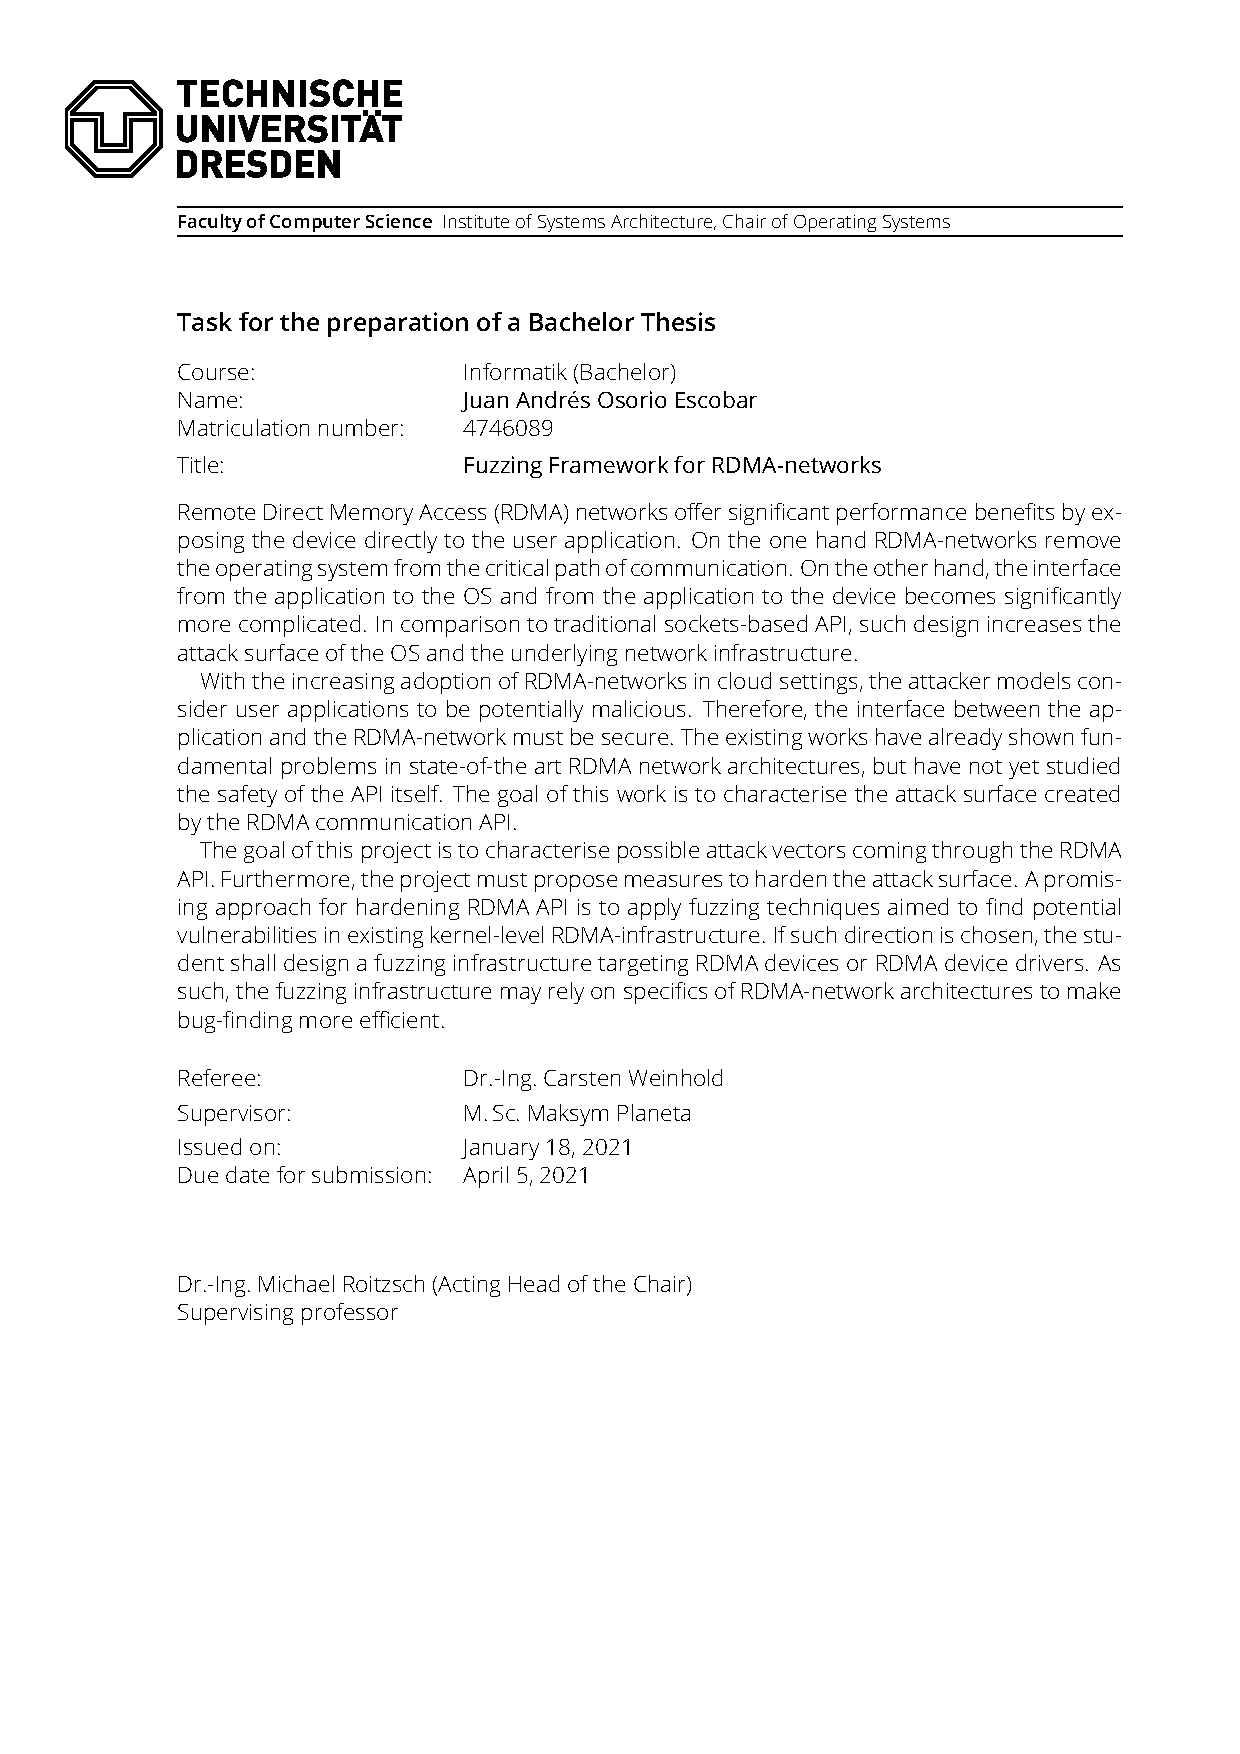
\includepdf[pages=-,pagecommand={},width=\paperwidth]{taskdescription.pdf}



%% \begin{justify}

%% Hiermit erkläre ich, dass ich die vorliegende Arbeit mit dem Titel \\


%% \vspace{0.5cm}
%%     \begin{center}
%%         {\large\sffamily\mdseries \@title } \\
%%         \vspace{1.0cm}
%%     \end{center}

%% selbstständig und ohne die Benutzung anderer als der angegebenen Hilfsmittel angefertigt habe. Alle Stellen, die wortwörtlich oder sinngemä\ss\ aus veröffentlichten oder nicht veröffentlichten Quellen entnommen sind, sind als solche kenntlich gemacht.\\


%% \vspace{2.5cm}
%% %\hfill \rule{0.33\textwidth}{0.4pt}\par
%% Dresden, \@date \hfill \@author
%% \end{justify}

%% \makeatletter
%% %% \chapter*{Selbstständigkeitserklärung}

%% \justifying Hiermit erkläre ich, dass ich die vorliegende Arbeit mit dem Titel \\

%% \vspace{0.5cm}
%% \centering
%% {\large\sffamily\mdseries \@title }
%% \vspace{1.0cm}
%% \justifying

%% selbstständig und ohne die Benutzung anderer als der angegebenen Hilfsmittel angefertigt habe. Alle Stellen, die wortwörtlich oder sinngemä\ss\ aus veröffentlichten oder nicht veröffentlichten Quellen entnommen sind, sind als solche kenntlich gemacht.\\

%% \vspace{2.5cm}
%% %\hfill \rule{0.33\textwidth}{0.4pt}\par
%% Dresden, \@date \hfill \@author
%% \makeatother

\newpage
\begin{center}
\textbf{\Large{Eidesstattliche Erklärung}}\\
\vspace{2cm}
\color{black}
Hiermit erkläre ich, dass ich die vorliegende Arbeit mit dem Titel
\vspace{1cm}

\textbf{Fuzzing Framework for RDMA-Network API} \\
\vspace{1cm}
\color{black}
\end{center}
selbstständig und ohne die Benutzung anderer als der angegebenen Hilfsmittel angefertigt habe. Alle Stellen, die wortwörtlich oder sinngemä\ss\ aus veröffentlichten oder nicht veröffentlichten Quellen entnommen sind, sind als solche kenntlich gemacht.\\


\begin{flushleft}
Dresden, 8. Mai 2021 \\
\begin{figure}[h!]
  \includegraphics[scale=0.45]{sign}
\end{figure}
Juan Andrés Osorio Escobar
\end{flushleft}


\begin{abstract}
  Nowadays, RDMA networks are being deployed in different environments which rely on high performance.
  The design of the network architecture of RDMA has  concentrated on performance, and previous works have
  proven that this design has inherent design flaws that expose
  various types of security concerns.

  In this paper, we focus on exploring the current implementation of the RDMA transport inside the Linux
  Kernel for implementation errors. To achieve this goal, we apply an efficient software
  testing technique that has discovered numerous bugs in different applications, namely fuzzing. The system call interface of the Linux
  Kernel and the network transmissions necessary for RDMA build the attack surface that we apply fuzzing on. For the system call interface, we
  use a popular system call-based Fuzzer named Syzkaller. For the network
  transmissions, we design a network architecture and implement an RDMA
  packet Fuzzer. Both approaches find memory errors and warnings in the
  RDMA infrastructure of the Linux Kernel.
\end{abstract}


\tableofcontents

\newpage

\listoffigures
\listoftables
\listofalgorithms
\lstlistoflistings


\section{Introduction}


% Computer Systems have become indispensable in our everyday life. Examples vary 
% from A to B. As they play important roles in our lives, we expect them to be 
% stable


\subsection{Goals}


% The main goal of this work is to provide an instrument to fuzz kernel modules
% in an enviroment in which kernel crashes are common. As a side goal, a better 
% understanding of fuzzing techniques and their reliablity should also be attained.

% TODO: move this back again to background

\subsection{The Linux Kernel}

% Linux distributions

One of the main features of the linux kernel is its ability to extend 
its functionality at runtime. Pieces of code that can be added (or removed) to the kernel 
while it is up and running are called moules. Each module is made of object code that can 
be dynamically linked with the insmod or modprobe executables\cite{ldd3}. 

Security checks in linux are enforced in the kernel code, if there are security vulnerabilities inside
the kernel, then the whole system has vulnerabilities.\cite{ldd3}

% Talk about the linux kernel being expandable by modules, which operate on
% so called `kernel space` or privileged mode, this makes them in turn mandatory
% to be well tested, because a malfunctioning module in this case a device 
% driver a potential target inside the system.


% TODO: explain that the kernel can be built with different configurations 


% In order to get a a custom kernel configuration that suits the needs of this work,
% the latest stable release (5.10.11 at the time of writing) was downloaded from kernel.org,
% the downloaded bundle contains the entire source code (called source tree) for the linux kernel.

% With this source tree, one can create a linux kernel, tailored down to a specific use case. In 
% this
When compiling the linux kernel, we want to enable support for the InfiniBand network stack, virtualization and 
also builtin functionality that will come to aid during the fuzzing process, the following are worth
mentioning:

\begin{itemize}
    \item Kcov: Code coverage for fuzzing. From \cite{kerneldocs-kcov} Kvoc exposes kernel code coverage information in a form suitable\
    for coverage-guided fuzzing (randomized testing). Coverage data of a running kernel is exported via\
    a debugfs file called kcov. % TODO:
    % NOTE ON KCOV profiling data will only become accesibleonce debugfs has been mounted mount -t debugfs none /sys/kernel/debug
    \item KASAN: The Kernel Address Sanitizer is a dynamic memory error detector. It provides\
    information for finding use-after-free and out-of-bound bugs, it uses compiler generated\
    instrumentation code to check every memory access \cite{kerneldocs-kasan} % TODO:
\end{itemize}

% As for all pieces of software, there are some requirements to build the kernel, 
% the list of programs needed for compiling the kernel are listed under \cite{minreqskernel}.

%Inside the kernel source tree main directory, running make causes the kernel build system to use the configuration 
%described inside a file named .config to build a kernel and all modules needed to support that configuration \cite{kroah-hartman06}.

\subsection{RDMA with Infiniband}

InfiniBand (IB) is a network architecture which provides very efficient and scalable server and storage interconnect
technology, which is capable of supporting Remote Direct Memory Access (RDMA). The IB technology enables data 
transmission between servers without needing CPU intervention,reducing in this way communication overhead, providing 
speeds going up to 56Gb/s per port\cite{rdmamanual}.

% TODO: Maksym: Should I talk about virtual protocol interface (VPI)?

\paragraph{RDMA over Converged Ethernet (RoCE)}

RoCE is a standard for RDMA over Ethernet, which allows leveraging RDMA semantics over an Ethernet network without needing
to resort to TCP transport. 
% According to \cite{rdmamanual} RoCE provided the most efficient low lattency Ethernet solution to the day of (their?) writing (in 2015).
% TODO: maksym => just say that RoCE is generally cheaper because it does not require specialized switches.
\paragraph{Rxe: Soft-RoCE}

Soft-RoCE is a software implementation of the RDMA transport (over Ethernet), it has been developed as a github 
community project, with help from IBM, Mellanox and other companies.This software driver provides us an 
uncomplicated manner to test RDMA technologies without needing to use real hardware, it provides a complete RDMA 
stack implementation over any NIC \cite{mellanox-community}.

% running \\ \$ modinfo rdma\_rxe \\ inside the shell, reveals that this module depends on the following modules: ib\_core, ip6\_udp\_tunnel, udp\_tunnel, ib\_uverbs 
% all which are as well loaded into the kernel when issuing the command \\ \$ modprobe rdma\_rxe \\
% modprobe loads a module into the kernel, while also loading the modules on which it depends on \cite{ldd3}.
% TODO: Maksym => this definitely does not go into the main body of the text, if you are so eager to conclude it, use appendecies.

% udev is a program that enables Linux to provide a persistent device-naming system
% in the /dev directory \cite{kroah-hartman06}

% To get Soft-RoCE capabilities, you need to install the kernel and user space libraries on both servers:
% We are mainly interested in the rdma\_rxe kernel module, Software RDMA over Ethernet, provides a software implementation of the RoCEv2 Protocol, cite manpages.


\subsection{Fuzzing}

Software testing is a tool used in software production pipelines, its main goal is to ensure proper program functioning. One common way to test programs is 
positive testing, in which these are tested against expected inputs under well defined scenarious (test cases), to produce the desired results.
Fuzzing is a technique used for negative testing, as opposite to the one just mentioned, in which the program is put under malformed or non-expected input. this
has lead to the discovery of many bugs in the recent years (TODO:\@ cite OSS website from lecture)

% The term Fuzzing was coined by Miller, as ... \ TODO: not so good bro.

\subsubsection{Types of Fuzzers}
 
Fuzzers can be categorized into 3 main types\cite{fetzer20}:

\begin{itemize}
    \item Blackbox: no knowledge of target program internals, therefore they have no means of measuring coverage and can only provide input to the target.
    \item Whitebox: these fuzzers rely on the knowledge of the source code of the target application, making them more efficient ( TODO: symbolic execution tools, model checkers that improve coverage, computed coverage guides the generator)
    \item Graybox: a combination of both blackbox and whitebox types.
\end{itemize}


\subsubsection{Coverage and Depth}

\subsubsection{Fuzzer components}

\paragraph{Generator}

\paragraph{Delivery method}

\paragraph{Monitoring Framework}

\subsubsection{Fuzzing Opensource Projects}

\paragraph{AFL}

\paragraph{Libfuzzer}

\paragraph{Syzkaller}

\paragraph{kAFL}
\section{background}



\subsection{RDMA Technology}


\subsection{The Linux Kernel}

Talk about the linux kernel being expandable by modules, which operate on
so called 'kernel space' or privileged mode, this makes them in turn mandatory
to be well tested, because  a malfunctioning module in this case a device 
driver a potential target inside the system.

\subsection{Fuzzing}

Software testing is a tool used used in software production pipelines, its main goal is to ensure proper program functioning. One common way to test programs is 
positive testing, in which these are tested against expected inputs under well defined scenarious (test cases), to produce the desired results.
Fuzzing is a technique used for negative testing, as opposite to the one just mentioned, in which the program is put under malformed or non-expected input. this
has lead to the discovery of many bugs in the recent years (TODO: cite OSS website from lecture)


\subsubsection{Types of Fuzzers}
 
Fuzzers can be categorized into 3 main types\cite{fetzer20}:

\begin{itemize}
    \item Blackbox: no knowledge of target program internals, therefore they have no means of measuring coverage and can only provide input to the target.
    \item Whitebox: these fuzzers rely on the knowledge of the source code of the target application, making them more efficient ( TODO: symbolic execution tools, model checkers that improve coverage, computed coverage guides the generator)
    \item Graybox: a combination of both blackbox and whitebox types.
\end{itemize}




\subsubsection{Coverage and Depth}

\subsubsection{Fuzzer components}

\paragraph{Generator}

\paragraph{Delivery method}

\paragraph{Monitoring Framework}

\section{Related Work}\label{s:related-work}


Research has categorized throughout the years the origins of
vulnerabilities inside the linux kernel. In 2001,~\cite{chouEmpiricalStudyOperating2001}
came to the conclusion that driver code has relative error rates
from 3 and up to 7 times higher than the rest of the kernel.

In 2011, an analysis from bugs ranging from january 2010 to march 2011
showed that 2/3 of errors originate from loadable modules\cite{chenLinuxKernelVulnerabilities2011}.

One interesting finding of~\cite{vanderstoepAndroidProtectingKernel2016} was that around 60\% kernel bugs
are reached from userspace by the ioctl system call.

The ioctl system call does not conform to any standard: the arguments, return values and semantics always vary
depending on the driver in question. It is commonly used as a catch all operations command for
operations that do not fit the UNIX stream I/O model.

One key aspect of the ioctl system call is it's intention to support generality by design.
Looking at its C prototype:

\begin{lstlisting}[language=c]
  int ioctl(int fd, int request, ... /* arg */);
\end{lstlisting}

The third (optional) argument serves as an untyped pointer to memory. This is implemented as a variadic argument, for at the time
the interface was designed, void* was not valid C. Nonetheless, the interface expects a single pointer, as opposed to potentially
many, which the variadic argument syntax would suggest.

\subsection{DIFUZE}\label{ss:difuze}

Acknowledging the fact that many of the functionalities to be fulfilled
by devices cannot be served through traditional system calls like read, write
and seek, DIFUZE is an interface aware fuzzing tool that targets
device drivers, by targeting the ioctl() interface\cite{corinaDIFUZEInterfaceAware2017}.
It was designed with the Linux Kernel for android devices in mind.

Commonly, handlers of ioctl calls are implemented as switch statements (on the second argument) which expect specific
input on the third argument. This poses a challenge for fuzzing, as this cross dependency constitutes a problem for extracting
the definitions of the expected data structures. There are tools that leverage taint tracking to recover input formats\cite{ganeshTaintbasedDirectedWhitebox2009}\cite{hallerDowserGuidedFuzzer2013}
but for ioctls, these techniques are not very effective\cite{corinaDIFUZEInterfaceAware2017} because they cannot recover this cross dependency between command identifier
and optional argument.

A naive approach could be to hook into the ioctl call on an application linked to the libibverbs library and mutate the arguments given to ioctl calls. Using techniques like the LD\_PRELOAD trick facilitates this,
but results are rarely successful because ioctl arguments are highly constrained in nature: An undefined request code
would most likely end in a default clause that serves for catching bad request codes. Randomly modifying the optional argument
without knowledge of its underlying structure is also not very likely to succeed.
Nevertheless, even though not very effective, this could still be a valid approach to target a potentially error prone interface.

Using static analysis, DIFUZE has overcome this difficulties by analyzing the source code of the device drivers,
collecting valid request codes and their corresponding data structures to be passed as a third parameter.

DIFUZE undergoes 3 main stages to achieve its goal:

\begin{itemize}
  \item \textbf{Interface recovery:} Analyze source code and detect enabled drivers. Identify which device files are used to interact with them, which ioctl handlers they have registered and what arguments they expect to be passed. This phase outputs a set of tuples in the form of ( device filename, ioctl command, structure type definitions ). It is noteworthy that the output of this stage can also be exported in a human readable .json file, making it easily reusable for other applications.
  \item \textbf{Structure generation:} Based on the definitions recovered from the previous step, this phase prepares conforming data structures to be passed to the actual execution environment.
  \item \textbf{On-device exection:} As already mentioned, DIFUZE was specifically designed with android devices in mind. Structures that were generated are passed to the component in the target device in charge of issuing ioctl commands, while maintaining a heartbeat signal as means of monitoring for system crashes.
\end{itemize}

DIFUZE was developed along with its own fuzzing engine called MangoFuzz, it is however integratable with other Fuzzers, like Syzkaller.

\subsection{Syzkaller}\label{ss:syzkaller}

Syzkaller is a grammar based, coverage guided unsupervised
system call fuzzer \cite{GoogleSyzkaller2021}. It is however not only
limited to Linux, but can also be used for Windows, BSD, among other
kernels.

The idea of Syzkaller is fairly simple, yet its implementation is very effective: it generates
programs consisting of a variable number of system calls, with
concrete arguments that are increasingly mutated across iterations.

Syzkaller's architecture consists of various components: An in-host manager, called
syz-manager which is in charge of starting virtual machines and persisting the programs that
reside on the input corpus which consist of short programs issuing
system calls. It is also in charge of generating crash reports, including a minimized C reproducer program of the crash and kernel console output (like KASAN reports, or panic
messages).

Inside the virtual machines, the syz-fuzzer process gets started by syz-manager. If an input
corpus exists, it is given to syz-fuzzer to guide the fuzzing process. Syz-fuzzer is
in charge of modifying programs and sending them to syz-executor. In Linux, programs that
are modified depend on coverage collected from kcov. Whenever a program seems to have triggered new coverage\footnote{code coverage generated by kcov is aimed to be stable, but false positives commonly refered to as 'flakes' may appear.},
it is executed repeatedly in order to make sure it does indeed trigger new coverage and is
afterwards sent back to the managing process to update the corpus.

Modifications made to programs are driven by heuristics and priorizations.\footnote{As with many other fuzzing projects, the inefficiency of searching through an enourmous space is made more bearable, by applying heuristics and priorization derived from experience: Do what usually works and not what does not likely trigger any bugs.}. Some of the highlights are\cite{vyukovSyzkallerAdventuresContinuous2020}:

\begin{itemize}
  \item Removing system calls might lead to new behaviour, but this is usually not the case. Adding new system calls to a program usually leads to higher coverages.
  \item Mutations on the arguments of a  system call with many and complex arguments are more likely to trigger new behaviour, than rather simple ones.
  \item Add system calls that are related to others, e.g. if a program already contains an open system call, a read or write system call on the file descriptor returned by open are more likely to trigger an error rather than say, the getpid or fork system calls.
\end{itemize}

\subsubsection{Specifying System Calls using Syzlang}

One of the core aspects of Syzkaller is the ability to declare system calls using
the system call description language Syzlang. Its goal is to function as a template
language for specify system calls based on extended types and specific or constant arguments,
e.g.\ open(``/dev/infiniband/uverbs0'', flags) is considered different system call from open(``/dev/null'', flags).

A great advantage of Syzlang is
that it allows to describe dependencies between system calls by using resources.
Resources are values that are meant to be passed from the output of one system call
into the input of another.
To illustrate why this is necessary, take for example the C function definitions found in the manpages:

\begin{lstlisting}[caption={Manpage C definitions for open and read}, language=c]
  int open(const char *pathname, int flags);
  ssize_t read(int fd, void *buf, size_t count);
\end{lstlisting}

Judging by only this declarations, it is not entirely clear that the result of open
is not any kind of integer, but one that plays the role of a file descriptor, similarly const char* is not
just any string, but a file\footnote{it is hard to rely on variable names, so `pathname' does not tell us much. Consider other system calls that use pathnames like chdir, where the variable name is just `path'.}. Furthermore,
it is not trivial to extract any interdependence between both calls for the same reason.

In contrast, syzlang declarations give a different type to this special kind of common types (int, const char*, etc.):

\begin{lstlisting}[caption={syzlang definitions for open and read}, label={lst:syzlangdefs}, language=c]
  open(file filename, flags flags[open_flags]) fd
  read(fd fd, buf buffer[out], count len[buf]);
\end{lstlisting}

By seeing both call declarations and knowing that open returns a file descriptor \emph{resource}, Syzkaller is aware
that this is resource needs to be passed as the first parameter to a read system call, and \textbf{not just any random integer.}

\subsubsection{Fuzzing Subsystems with Syzkaller}

Syzkaller can be configured to use only a subset of all system calls, which are all defined under
the /sys/\textless~architecture\textgreater/ directories. This configuration allows syzkaller to fuzz
a specific subsystem in the kernel. With this information one can target specifically
the infiniband RDMA subsystem of the kernel.

\subsubsection{Mellanox and Syzkaller}

On the Linux Plumber's conference of 2018, Mellanox\footnote{Mellanox is also mostly in charge of the development  of verbs userspace libraries libibverbs.} --- one of the biggest suppliers of RDMA enabled hardware,
presented their collaboration with the head Syzkaller
developer Dmitry Vyukov, with the goal of expanding syzkaller subsystem definitions with system calls
that are handled by RDMA device drivers\cite{osherovichImprovingTestingRDMA2018}.

Following this conference, an extensive description of the RDMA subsystem was incorporated into Syzkaller's repository on github.

Mellanox acknowledged during this conference that they use Syzkaller for internal testing,
and also mentioned running syzkaller over SoftRoCE, it will crash almost immediatly. From this, it is clear
that this method is highly effective and that RDMA drivers may still contain various implementation errors.

\subsection{Fastsyzkaller}\label{ss:fastsyzkaller}

By using a probabilistic model called N-Gram model, patterns of system calls sequences are marked as vulnerable based on their appearance and
frequency inside programs that cause crashes. In the natural language processing domain, an N-Gram is defined as a subsequence
of n words; in this case it is refered to a sequence of n system calls that appear on a program. Using the chain rule
of probability, the likelihood presence of the nth word can be calculated, given the n-1 previous words (system calls)\cite{jurafskySpeechLanguageProcessing2000}.

By letting syzkaller run for two weeks, an initial input corpus of programs is generated. Based on this input corpus,
patterns of syscalls with length n are extracted from programs that cause crashes, and are marked as vulnerable
patterns. The authors found the fixed value of n = 5 to be the most effective\cite{liFastSyzkallerImprovingFuzz2019}.
Based on these five-gram patterns, new test cases were generated and introduced into the corpus.

Equiped with this preloaded corpus, slight modifications are made to the test case generation algorithm in order
to enforce and preserve the presence of vulnerable system call patterns in programs. These modifications are:

\begin{itemize}
  \item The algorithm can only insert system calls which are marked as being high priority, dictated by the probability given by the N-Gram model.
  \item The algorithm cannot remove or mutate system calls in a given sequence that is part of a vulnerable pattern.
  \item The algorithm cannot splice test cases, as this might remove the presence of vulnerable patterns.
\end{itemize}

Fastsyzkaller was found to be 3 times more effective in bug finding than syzkaller during a 4-week time period.
By analyzing the programs generated by RDMA-syzkaller, one can see that many of the programs that do not generated are very short, consisting
of 1 - 2 system calls, where programs that generate crashes are at least 3 system calls long. Specifically fuzzing the RDMA subsystem using this
approach can provide efficiency gains.

\subsection{Network Protocol Fuzzers}\label{ss:network-fuzzers}

Another valid approach to put RDMA related drivers under stress is to target the network packets these drivers
parse and process. This Subsection presents Open Source Fuzzers which specifically target network procotols.

\paragraph{}\textbf{Mutiny}~\footnote{\url{https://github.com/Cisco-Talos/mutiny-fuzzer}}
is a tool that uses captured packages (PCAP files)
to replay and modify legitimate traffic and send it to a target
application. Mutiny relies on radamsa, a simple black-box fuzzer, to mutate packets.

\paragraph{}\textbf{Sulley}~\footnote{\url{https://github.com/OpenRCE/sulley}} is a fuzzing library / framework that allows for highly automated fuzzing.
Sulley provides abtract classes that aid in the implementation of a
monitoring framework. The monitoring framework restarts the target
application in case of crashes. Sulley will try to reproduce crashes
by resetting the target into a healthy state and resending the last packets
before the crash was detected. It starts with the last packet and steps
back until it finds the sequence of packets that triggered the crash and
proceeds to record this data. It was designed for a Windows environment and
is unfortunately not under active maintenance.

\paragraph{}\textbf{BooFuzz}~\footnote{\url{https://github.com/jtpereyda/boofuzz}} is the active fork of Sulley. Unlike Sulley, BooFuzz has better
support for a Linux host environment and for monitoring Linux virtual
machines. It provides more alternatives for fuzzing, including support for
ethernet and IP layer fuzzing. Although it provides help for implementing
core aspects of fuzzing like monitoring and recording of data (like
Sulley), it has a learning curve it demands of the user to
implement many details by herself.

\paragraph{}
These tools offer either limited control over granularity of packet field
modifications, or demand from the Fuzzer developer thorough protocol
definitions and instantiation of packet objects for the frameworks to
use (in case of Sulley/BooFuzz). These limitations are described in
more detail in Section~\ref{ss:prob-nw-fuzzers}.

\section{Design}\label{s:design}

%% First motivate your architecture
%% > Why did you chose proxy architecture
%% > Why in one direction
%% > What kind of problem do you try to solve, others dont
%%
%% Then explain how it works
%%
%% then xplain what useful new properties you get
%%
%% do not forget coverage information: say one
%% needs it in principle, but in the implementation
%% I can say I did not do it, because of time constraints.

We want to address specific challenges that arise when fuzzing
RDMA appications. We have seen in Subsection~\ref{s:ibverbs-challenges}
that to test specific parts of the code, the RDMA API requires a connected environment, i.e.
that an application has a Queue Pair that reaches one of the ready states; otherwise,
the code of the device driver in charge of processing RDMA traffic will branch out
to simply drop the traffic and many code paths will remain untested.

\subsection{A Proxy Architecture}

A sensible choice for testing connected applications is to
target the communication channel that these applications use.
A proxy architecture allows a process to sit in the middle of two applications
and read and/or modify the traffic before forwarding such traffic to the original destination.
We will refer to this process in the middle as the proxy fuzzer. Simply put, the proxy fuzzer
takes incoming traffic from an RDMA application and forwards it to another RDMA application.
In doing so, the proxy fuzzer can modify the traffic in such a way that it specifically targets the RDMA stack of a target machine.

\begin{figure}[h]
   \centering
   \includegraphics[width=\linewidth]{proxyfuzzerconcept}
   \caption[Proxy fuzzer concept]{Basic concept of a Proxy fuzzer, the red arrow denotes fuzzed traffic.}\label{fig:fuzzerconcept}
\end{figure}

Figure~\ref{fig:fuzzerconcept} depicts the concept of this architecture. Because we also want to be able to differentiate
easily which packets may cause specific errors, we separate the applications into two different environments by
using two virtual machines. In case of a kernel panic or any other kind of crash, the host environment remains unaffected
and can retain the series of packets that were responsible for triggering the crash.

The fuzzer only modifies the packet headers of RDMA traffic, because it is concerned
with testing the RDMA stack and the RDMA stack only. Thus, the Base Transport Header and Header extensions
are the actual fuzzing targets.  If the proxy fuzzer were to modify IP or Ethernet Headers,
the packets would most likely not reach their destination. Fuzzing other
network protocols is out of the scope of this work. The RDMA payload is completely ignored,
because RDMA device drivers are also not concerned with it. % TODO:\@ As we have already said this work is mainly concerned with fuzzing rdma with softroce as our entry point (or something similar)

Figure~\ref{fig:fuzzerconcept} shows that the traffic is fuzzed only in one direction. The reason
behind this is the nature of network protocols. Traffic for network protocols must conform to an underlying
structure and excessive header manipulations usually just leads to dropped packets. The code coverage information provided by
kcov is collected from the target machine by transmitting coverage information through the network. Code
coverage information is, as we have mentioned, an important aspect of efficient bug discovery.

\subsection{Advantages of this Approach}

By having knowledge of the Protocol, the proxy fuzzer can make conscious modifications to fields in the Base Transport
Header (See Table~\ref{tab:bthfields}), in the hopes of encountering bugs. We refer to conscious modifications here,
because some fields are required to always have specific values (e.g. Transport Header Version), these fields must remain unmodified.

The main advantage is that with this architecture, the proxy fuzzer is able to test code paths
that were previously untested by the tools presented in Subsections~\ref{ss:difuze},~\ref{ss:syzkaller}~and~\ref{ss:fastsyzkaller}.

It is relevant to mention that even though this design was conceived with
SoftRoCE at hand, it can be applied to anything that processes Base
Transport Headers, even real RDMA-enabled NICs. This is true because processing of
Base Transport Headers is implemented at the hardware level.



%% To specifically target the RDMA network stack,
%% We can connect two RDMA applications in different machines and





%% Mention that the goal of this design is to test the driver.
















































%% Since many state-of-the-art fuzzers do not directly address some of the challenges
%% posed by RDMA applications (see Section \ref{s:ibverbs-challenges}), I propose a fuzzer that plays the role
%% of a proxy between two machines which comunicate using RDMA. The network architecture
%% allows the fuzzer not only to monitor traffic between the machines, but also to modify it.
%% Unlike system call based fuzzers, this approach can easily test code paths which require
%% fully initialized and connected applications, in the context of RDMA Verbs. % ibverbs.

%% As the goal of the fuzzer is to trigger bugs related to the RDMA network stack,
%% only the modification of headers that are pertinent to it is desirable;
%% the Base Transport Header, sitting at layer 4,
%% defines fields relevant to RDMA applications (see Table \ref{tab:bthfields}). Fuzzing any other headers such as
%% ethernet or IP headers would be detrimental to efficiency, as other parts of the network stack may not be able
%% to deliver the packets; the modified packets would
%% not even reach the target application. Fuzzing payload contents is also undoubtedly inefficient,
%% because it does not concern RDMA device drivers.

%% It is relevant to mention that even though this design was conceived with
%% SoftRoCE at hand, it can be applied to anything that processes Base
%% Transport Headers, even real NICs. This is true because processing of
%% Base Transport Headers is implemented at the hardware level. %% maybe cite this?

%% \begin{figure}[h]
%%   \centering
%%   \includegraphics[width=\linewidth]{proxyfuzzerconcept}
%%   \caption[Proxy fuzzer concept]{Basic concept of a Proxy fuzzer, the red arrow denotes fuzzed traffic.}
%%   \label{fig:fuzzerconcept}
%% \end{figure}

%% Figure \ref{fig:fuzzerconcept} depicts the conceptual architecture for the Proxy Fuzzer.
%% The traffic can be fuzzed in any direction, including both directions simultaneously.
%% Nevertheless, as network protocols must conform to an underlying structure and excessive header manipulations usually
%% just lead to dropped packets, the conceptual
%% design is mainly concerned with fuzzing in one direction, as shown in figure \ref{fig:fuzzerconcept}.

\section{Implementation} % maybe this is still part of design

To carry out the network architecture that will allow us to seamlessly read and modify
network traffic, as proposed in section \ref{s:design}, we can use the combination of
`quick Emulator` QEMU and the Kernel-based Virtual Machine (KVM) as a virtualizer. The qemu-system command which
starts a virtual machine allows us to specify parameters such as:
\begin{itemize}
  \item The kernel boot image,
  \item Disk image files from which we can provide a prepared file system, % TODO: which contains the installed modules for RDMA and the latest iproute2 version to enable software rdma devices,
  \item Virtual network interfaces.
\end{itemize}

\subsection{Setting up the Network}

QEMU can create a virtual network device
inside the guest environment (e.g. a PCI network interface) and we can specify a backend to the
guest network interface. This backend is a virtual network interface that interacts with the
emulated NIC:\@ it puts the packets from the guest into the host and vice-versa\cite{DocumentationNetworkingQEMU}.

A TAP device is a virtual interface that provides packet reception and transmission for user space programs.
TAP devices operate on the data link layer, they carry ethernet frames.
A TAP device can be created from a user program by opening the device `/dev/net/tun'  and issuing a
corresponding ioctl() call to register a new interface with the kernel\cite{krasnyanskyUniversalTUNTAP}.
Listing \ref{lst:tapifr} shows a snippet demonstrating how to register/open a TAP device.

%% snippet of the open and ioctl call.
\begin{lstlisting}[caption={Registering/opening a virtual TAP interface}, label={lst:tapifr},  style=CStylespecial]
 #include <linux/if.h>
 #include <linux/if_tun.h>

  /* inside register/open device function */
  struct ifreq interface_req;
  int fd, err;

  fd = open("dev/net/tun", O_RDWR);

  /* check for errors */
  /* ... */

  memset(&interface_req, 0, sizeof(interface_req));
  interface_req.ifr_flags = IFF_TAP;
  interface_req.ifr_name = "tap0";

  err = ioctl(fd, TUNSETIFF, (void *) &interface_req);

  /* check for errors */
  /* ... */

  return fd;
\end{lstlisting}

Normally, the registered TAP device disappears as soon as the process that created the interface exits, but
the interface can be made persistent with a further ioctl() call. Persistent interfaces can be opened
by another process by issuing the exact same open() and ioctl() calls as when registering the interface
for the first time.
%This is part of what the ip tuntap command does\footnote{iproute2: https://git.kernel.org/pub/scm/network/iproute2/iproute2.git/ }
A TAP interface is the type of backend we associate to the VM's network interface. However, a problem arises
when we trying to open the TAP devices that are associated with the QEMU process: the ioctl() call
fails and sets the global error variable ERRNO to EBUSY (device or resource busy). When
we dig into the kernel sources for the functions that handle registration and attachment for this type of device,
we see that the operating system returns  this error when the user registers a device without multiqueue support and this device was already
attached\footnote{Under a recent Linux Kernel source tree, see drivers/net/tun.c: specifically tun\_set\_iff() and tun\_attach() }.
We are not interested in enabling multiqueue support, as ...

We can connect the TAP device associated with the QEMU process to a virtual bridge, and connect an additional TAP interface to the bridge.
For each VM, we create then an additional TAP device and a bridge. In this way, we can open the additional tap devices within our fuzzer
process. Figure \ref{fig:networkdetailed} shows the layout of the network architecture we describe.

\begin{figure}[h]
  \centering
  \includegraphics[width=\linewidth]{proxyfuzzernetworkdetailed}
  \caption[Proxy fuzzer network architecture]{Detailed network architecture for the proxy fuzzer}
  \label{fig:networkdetailed}
\end{figure}

Now that we can open the interfaces labeled as tap1 and tap2 in figure \ref{fig:networkdetailed}, we ``connect'' the
network by forwarding the traffic from tap1 into tap2 inside the fuzzer process, and vice-versa. The fuzzer
process takes a frame by simply calling read() on the TAP device and forwards it to the other device by calling write().
Listing \ref{lst:fwdtraffic} shows how the porcess forwards traffic in one direction. The other direction is handled by a
child process in an analogous manner.

\begin{lstlisting}[caption={Forwarding traffic in the proxy fuzzer process}, label={lst:fwdtraffic},  style=CStyle, float, floatplacement=H]
  /* file descriptors for tap1, tap2 interfaces */
  int fd_tap1, fd_tap2;

  /* open the interfaces */
  /* ... */

  /* infinite forwarding loop */
  while (1) {
    /* take frame from interface tap1 */
    read_from_tap1 = read(fd_tap1, buffer_tap1, BUFFER_MAX_LEN);

    /* do something with the frame */
    /* ... */

    /* put the frame into interface tap2 */
    write(fd_tap2, buffer_tap1, l);
  }
\end{lstlisting}

\subsection{Preparing the Guests' Environment}

We want to prepare a basic Linux system with support for RDMA and SoftRoCE.
To accomplish this we mount a blank file into our file system and use the tool
debootstrap to install a debian distribution inside the mount point directory.
We can specify a list of packages that debootstrap will install into the system,
so that we can do the following:

\begin{enumerate}
  \item Build RDMA applications using the libibverbs library,
  \item Create a virtual rdma device over an existing interface: this requires a recent version of the iproute2 package,
  \item Build and run performance benchmarks for RDMA applications.
\end{enumerate}

We also install the modules required for SoftRoCE and RDMA into this file system.
For simplicity, we took out the header checksum validation inside of the SoftRoCE module. We consider
this is not too invasive, because we could also achieve the same results by recomputing the checksum values after modifying
the headers and writing the new value into the header.
The kernel we use is compiled with the options described in Subsection \ref{ss:fuzzingkernel}.

\subsection{Fuzzing the Traffic}

The Proxy fuzzer parses the frames read and determines wether it carries RDMA traffic, i.e. a Base Transport Header.
If there is RDMA traffic, the fuzzer mutates a random field of the header (see Table \ref{tab:bthfields}), with the following exceptions:

\begin{itemize}
  \item Transport Header version, because the SoftRoCE driver enforces the requirement of this field always being equal to 0: if its not, SoftRoCE will drop the packet.
  \item Destination QP, because when there is no Queue Pair with a matching number, the packet will also be dropped.
\end{itemize}

After fuzzing the Base Transport Header fields, the fuzzer will check wether the OpCode determines the presence of Header Extensions,
which the fuzzer will try to parse accordingly and modify as well.

The Fuzzer modifies the fields by generating a random byte (ranging from 0x00 to 0xFF) and
assigns to a random header field the result of such header field XOR'd with the random byte. This is done a random number
of rounds, with a limit of 3 rounds per packet. It can occur that the fuzzer leaves the packet intact if the number of rounds is zero.
Algorithm \ref{alg:fuzz} outlines this procedure.

\RestyleAlgo{boxruled}
\SetAlgoVlined
\begin{algorithm}[t]
  \caption{A Simple Algorithm for Fuzzing RDMA Headers}
  \label{alg:fuzz}
  \LinesNumberedHidden
  \DontPrintSemicolon
  \KwIn{An Array of bytes $Packet$, a number of rounds $n \leq 3$}
  \KwOut{A modified Array of bytes $Packet$}
  $MaxHeaderOffset \gets 12$\;
  $MaxByteValue \gets 255$\;

  \For{$i \gets 1$ \textbf{to} $n$}{
      $randomByte \gets Random()  \; \% \;  (MaxByteValue + 1)$
      $randomOffset \gets Random() \; \% \; MaxHeaderOffset $
      $Packet[randomOffset] \gets Packet[randomOffset] \oplus randomByte$
  }
  $OpCodeOffset \gets 0$\;

  $OpCode \gets Packet[OpCodeOffset]$\;
  $OpCodeWithHeaderExtensions1 \gets 0$\;
  $OpCodeWithHeaderExtensions2 \gets 1$\;
  \Switch{OpCode}{
    \Case{OpCodeWithHeaderExtensions1}{
      $Packet \gets FuzzHeaderExtensions(Packet, OpCode)$
    }

    \Case{OpCodeWithHeaderExtensions2}{
      $Packet \gets FuzzHeaderExtensions(Packet, OpCode)$
    }
    /* More cases for OpCodes with header extensions */\;
    /* ... */\;
    \Other{
      nothing
    }
  }

  \Return{Packet}
\end{algorithm}

After fuzzing a packet, the Fuzzer will write the resulting header into a log file for error reproducibility.

TODO

\section{Discussion}
%% talk about findings of Syzkaller and proxy fuzzer

%% talk about other tools for fuzzing network protocols and why they were not so relevant (act as clients)
%% Other tools problems:
%% BooFuzz:
%%  * is either a client or a server. different instances of (Fuzzable) communication per channel. => this is seamlessly done with proxy fuzzer
%%  * must provide packet content from scratch and let the application know which fields it can fuzz. impractical because different packet anatomies.
%%  * Even though it is easy to install, bla bla von oben. SEITE VERLINKEN.
%%  * does not provide coverage support out of the box.
%%  * multiple sessions for each communication channel => awkward to establish a connection.
%%
%%  The network architecture that Proxy Fuzzer has is far more convenient, because:
%%    * Test connected applications, QP already in ready state.

\subsection{Difficulties with other Tools}

Some tools were mentioned in Section~\ref{s:related-work} but could not be evaluated in Section~\ref{s:evaluation}.
Despite this, we consider them to be interesting approaches that build on top of state-of-the-art tools and techniques.

\subsubsection{Fastsyzkaller}

Unfortunately, Fastsyzkaller's authors did not release any source code of their contributions to open source.
It would have been difficult to reimplement Fastsyzkaller under the time frame given and also explore
other approaches.

Nevertheless, we examined the programs created by Syzkaller and compared them to programs that generate crashes.
Syzkaller serializes programs into a specific binary format and saves them in a binary file called corpus.db.
Extracting the programs required us to extend Syzkaller with a module that dumps all programs in the corpus into a file.
The output file contains all programs inside the corpus separated by a marker string.
% MAKSYM: show some program outputs???
From this information, we can see that most of the programs generated by Syzkaller are one, two or three system calls long.
The minimized versions of the programs which caused crashes consist of two to four system calls. This suggests
that errors occur with programs that tend to be longer than most programs generated by Syzkaller.
In contrast with Syzkaller, Fastsyzkaller runs a modified generation algorithm, which is inclined to create programs
with more system calls (See Subsection~\ref{ss:fastsyzkaller}).

We consider that further exploring the N-Gram model, as a tool for recognizing vulnerable system call patterns could bring
efficiency gains. As we said, some bugs found by syzkaller are only caused by programs that consist of two system calls;
these kinds of bugs are more likely to be shallow bugs, as opposed to bugs that require a very specific program state
originating a sequence of different system calls with specific arguments.

%% LONG SYZKALLER PROGRAM TRIGGERING CRASH THAT WAS NOT REPRODUCEABLE. QP CREATION, QUERY MR AND ALL THE GOOD STUFF, VERY INTERESTING.

\subsubsection{DIFUZE}\label{ss:disc-difuze}

Inside the Syzkaller's source tree, comments containing TODOs inside the Syzlang definitions of the RDMA subsystem (``syz/linux/rdma.txt'') and
the presence of only three ioctl system call definitions led us to think that using DIFUZE for generating ioctl interface definitions
was a very promising path. The generated .json files that contain correct ioctl definitions could have been easily ported into the
Syzlang specification of the RDMA subsystem inside of Syzkaller. This could have improved Syzkaller's performance at fuzzing
the RDMA subsystem.

Despite our numerous efforts to generate interface definitions for ioctl calls by using DIFUZE,
everything we tried failed. Even though the authors provide a Docker image containing all dependencies
to run DIFUZE, the version of clang used by the authors (3.8.1) was unable to recognize
many compiler arguments of newer versions of gcc whith which the kernel was compiled. This is an essential step
for DIFUZE because it requires the exact compilation command that was run by make.
%% MAKSYM: it requires the exact compilation command that was run by make =: correct? .
After updating clang and llvm to the latest versions available at the time of this writing (13.0.0), the routine in charge of
the first stage of DIFUZE (interface recovery) ran until completion, albeit with many similar warnings
to those raised by earlier versions of clang/llvm.

Unfortunately, even though this interface recovery routine
was able to complete, there were no output files for any of the drivers that were compiled, including SoftRoCE and
RDMA core modules. The routine reports it has found zero ioctl functions to process.

\subsection{Limitations of Other Network Protocol Fuzzers}\label{ss:prob-nw-fuzzers}

We have mentioned in Subsection~\ref{ss:network-fuzzers} other tools for fuzzing network protocols: Sulley, its successor
BooFuzz and Mutiny. In the case of Sulley and
BooFuzz, we did not use these tools because we found some limitations with them:

\begin{enumerate}
   \item The user must provide a definition of the network protocol, she must also instantiate the packets that the fuzzer will modify from scratch. The result of the fuzzing with this tools is heavily dependant on this input. The Proxy Fuzzer operates on packets created from actual connected applications, removing the unnecessary effort of instantiating packets. The Proxy Fuzzer can easily test different layouts of RDMA packets, you just need to change the applications. In our case, this allowed us to conveniently run different benchmarks and test different types of header combinations (Base Headers plus Header extentions).\label{enum:d-1}
   \item They are by design, communication endpoints; they act either as the client or as the server. This presents an awkard situation because RDMA applications need to exchange information first before they can connect with each other through the actual communication channel. This means that the library user would have to craft the packets required for exchanging information and send them either through a different session instance in the tool (or send them outside the tool and then start it)  and then switch to the other channel to start the fuzzing with packets which also have to be crafted by the user. This seems rather clumsy in comparison to the seamless approach of the Proxy Fuzzer.\label{enum:d-2}
   \item They do not provide support for coverage collection, therefore they also do not have coverage-guided test case generation.\label{enum:d-3}
\end{enumerate}

Although limitation~\ref{enum:d-3} also holds true for the Proxy Fuzzer, we consider that the Proxy Fuzzer is more adequate for
targetting the RDMA stack because it does not suffer from the disadvantages of limitations~\ref{enum:d-1} and~\ref{enum:d-2}.

Mutiny is a tool that uses captured packages (PCAP files) to replay and modify legitimate traffic and send it to a target application.
It does not provide the fine grained control that Proxy Fuzzer implements through bitmasks for header manipulations, that let us fuzz
specific bits containing fields while leaving other fields intact. This for example necessary in the case of the fields Solicited Event,
MigReq, Padcount and Transport Header Field (see Table~\ref{tab:bthfields}) because they all lay on the same byte. We remind that we want to
leave the Transport Header Field intact. Mutiny does
not implement support for switching communication channels, which is similar to limitation~\ref{enum:d-2}.

Nevertheless, with some effort and some modifications, these tools could have also been integrated
into the Proxy architecture, replacing the Proxy Fuzzer to some extent. It is possible that in integrating them, the fuzzing process would have yielded better results.


\subsection{Future Work}

As mentioned in the previous subsection, the results with incorporating
existing network protocol fuzzers into the proxy architecture were
not explored. Specifically, writing glue code to integrate BooFuzz into the architecture would
be the most promising path, since it is the only actively maintained project and allows fine grained control over modifiable fields.


\subsubsection{Proxy Fuzzer}

There were some aspects of state-of-the-art Fuzzers that we could not implement, given the time constraints.
Efficient Fuzzers are complex long-time projects involving many experienced developers. Important features were left
because of this for future work, these were:

\paragraph{A Monitoring System} in charge of synchronizing the applications that communicate with each other,
as well as monitoring the target to detect crashes automatically. The Monitoring System would communicate
with a process inside the virtual machines via RPC, which would start or restart the application whenever necessary.
In the current setting, the applications must be restarted by hand whenever one side terminates the communication either by crashing
or gracefully exiting from user space. The Monitoring System would maintain a heartbeat signal with the machines, so that it knows when they have
crashed; this signal could be implemented with something simple like the Ping network utility.
They must also be restarted when the test is complete. Whenever a machine crashes, the Monitoring
System could also be in charge of two important tasks:

\begin{itemize}
\item Bring up the crashed machine by issuing the respective qemu-system command,
\item Notify the Proxy Fuzzer instance of the crash.
\end{itemize}

\paragraph{Output for Error Reproducibility:} when The Proxy Fuzzer is notified of the event of a crash, it can dump all
RDMA traffic that it forwarded since the applications started communicating, and additionaly include the crash information
that would be provided by the Monitoring System.

\paragraph{Code Coverage Collection from Kcov:} This is an essential aspect for efficient generation of test cases.
In the context of the Proxy Fuzzer, this would shed light into which header field modifications trigger more
code paths than others. With this information, we could tune Algorithm~\ref{alg:fuzz} to adapt and focus
more on header modifications that are more likely to dismantle bugs.

\subsubsection{Syzkaller}

Syzkaller is still to the date of this writing an active project that follows the development of the Linux Kernel development
branches~\cite{shiIndustryPracticeCoverageguided2019}. Syzkaller benefits from academic
research and will continue to do so in the future, it is the center of recent research works
(~\cite{kim2020hfl},\cite{hongNovelDynamicAnalysis2021} and~\cite{pailoorMoonShineOptimizingOS2018}).
For all these reasons, it is sensible to put effort into developing a more specialized framework for continuous fuzzing
of the RDMA stack based on Syzkaller, which could be similar to the proposal of~\cite{shiIndustryPracticeCoverageguided2019}.

% UGLY
%% For all this reasons, it is a reasonable approach to develop a continuous Fuzzing Framework
%% based on Syzkaller, as proposed by~\cite{shiIndustryPracticeCoverageguided2019}.

The results of fuzzing are correlated with the quality of the seed/input files~\cite{liangFuzzingStateArt2018}.
In the case of Syzkaller, the starting point (seed) for test case generation is the set of definitions
provided through the Syzlang language. As we have seen in Subsection~\ref{ss:disc-difuze}, there is
a possibility that the RDMA subsystem Syzlang definitions could be improved.

\section{Conclusion}

I conclude working copy is actually not bad

\bibliographystyle{acm}
\bibliography{references.bib}
\appendix 
\section{Building and Configuring the Linux Kernel}



\end{document}
